\FloatBarrier
\newpage
\onecolumn
\appendix

\begin{center}
{\Large \textbf{APPENDIX}}
\end{center}
\addcontentsline{toc}{section}{APPENDIX}

\section{Supplementary Materials}
\label{sec:appendix}

This appendix provides supplementary visualisations referenced in the main text, organised into six sections: (A.1)~confusion matrices for all four models, (A.2)~EDA distribution plots, (A.3)~the detailed process flow diagram, (A.4)~per-class word clouds, (A.5)~web application interface screenshots, and (A.6)~ablation study visualisations.

%% ── A.1  Confusion Matrices ──
\needspace{20\baselineskip}
\subsection{Confusion Matrices}

Figure~\ref{fig:confusion_matrices} presents the full set of confusion matrices. The Joy$\leftrightarrow$Love and Fear$\rightarrow$Surprise misclassification patterns persist across all architectures, confirming that semantic overlap --- rather than model capacity --- is the primary classification bottleneck. XGBoost~(d) additionally exhibits majority-class bias, with elevated Sadness$\rightarrow$Joy and Anger$\rightarrow$Joy off-diagonal counts.

\begin{figure}[H]
\centering
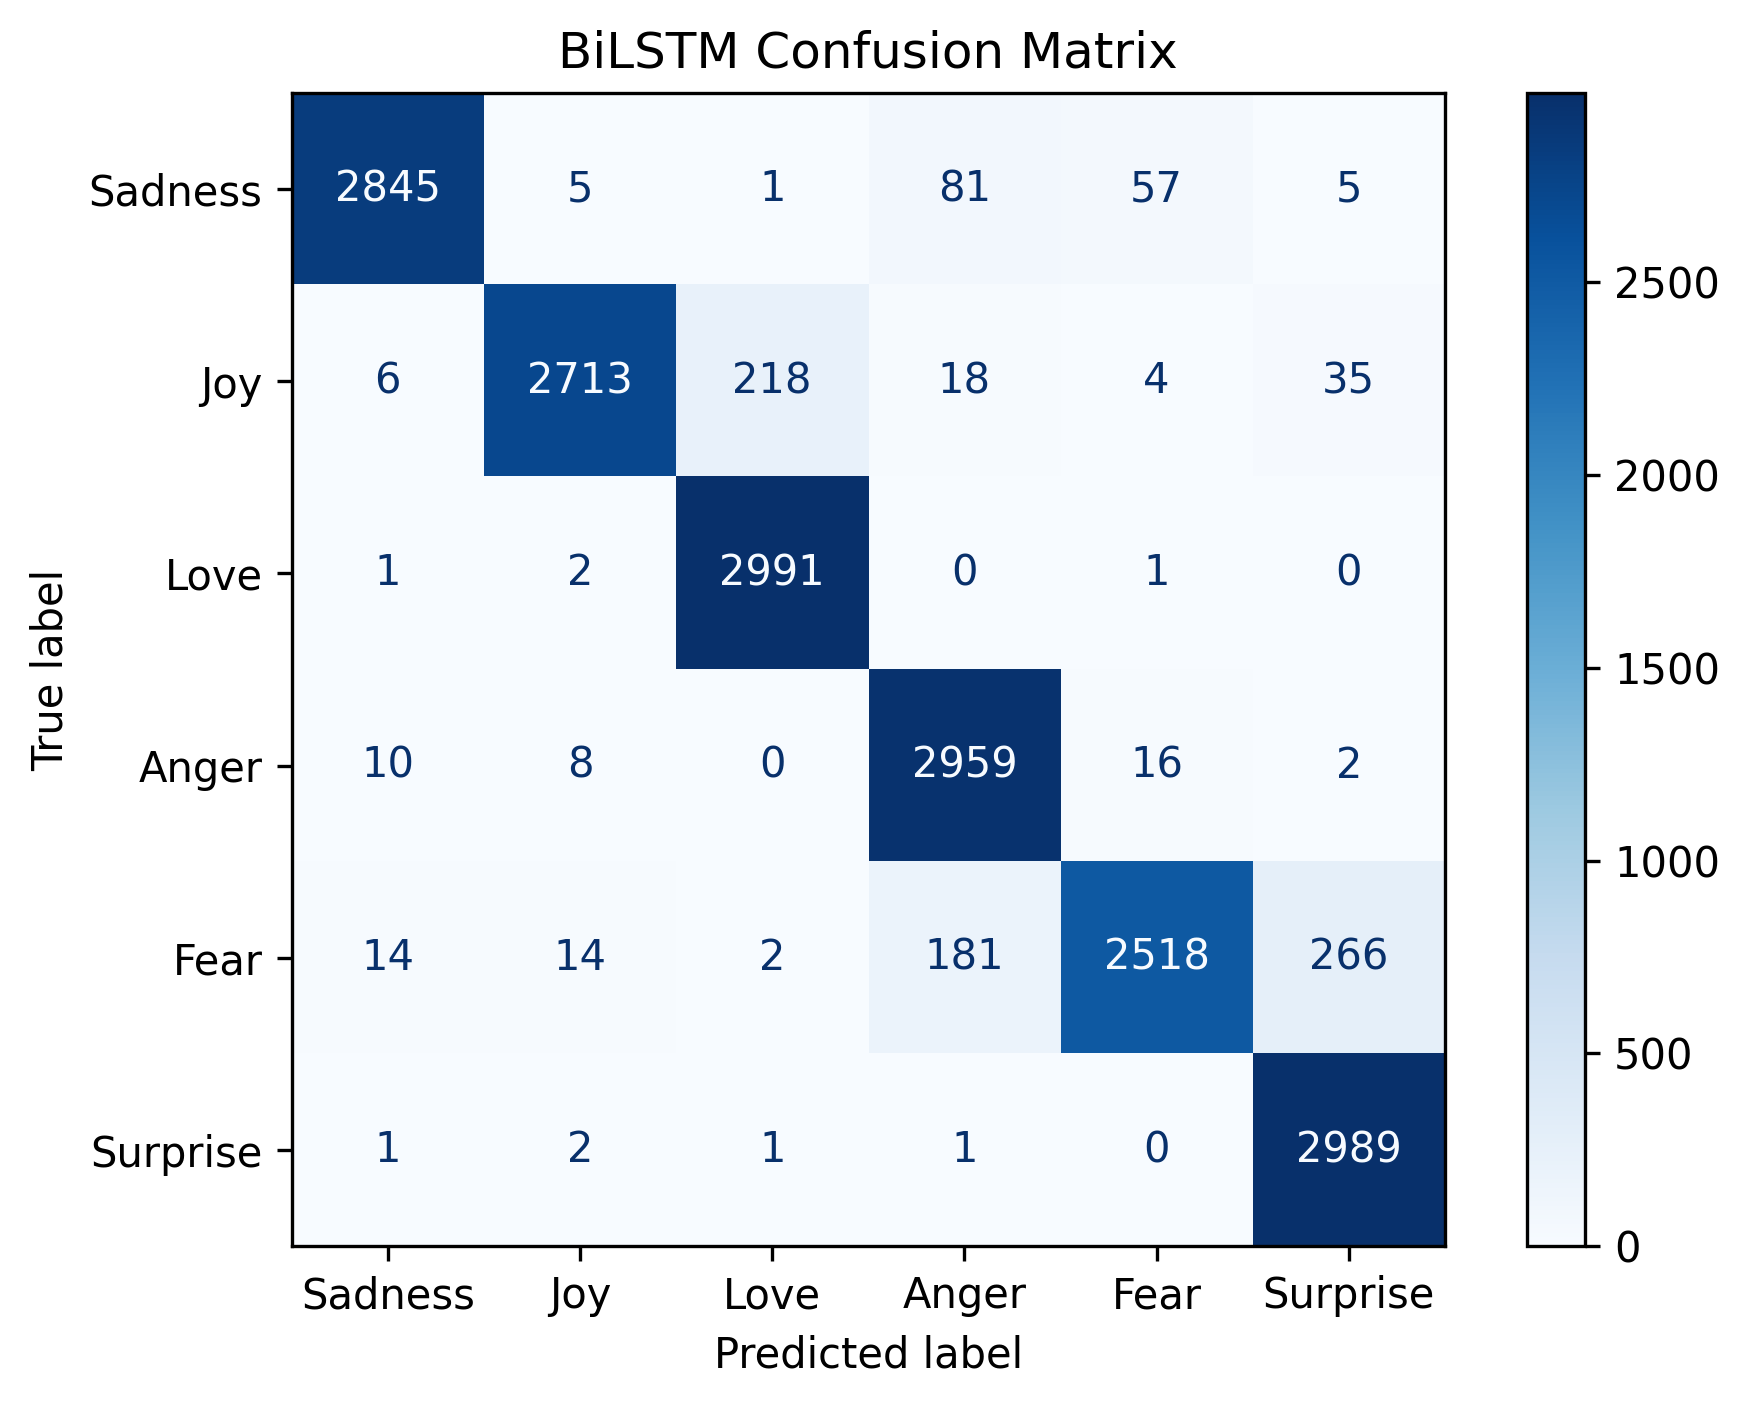
\includegraphics[width=0.48\linewidth]{figures/bilstm_confusion_matrix.png}\hfill
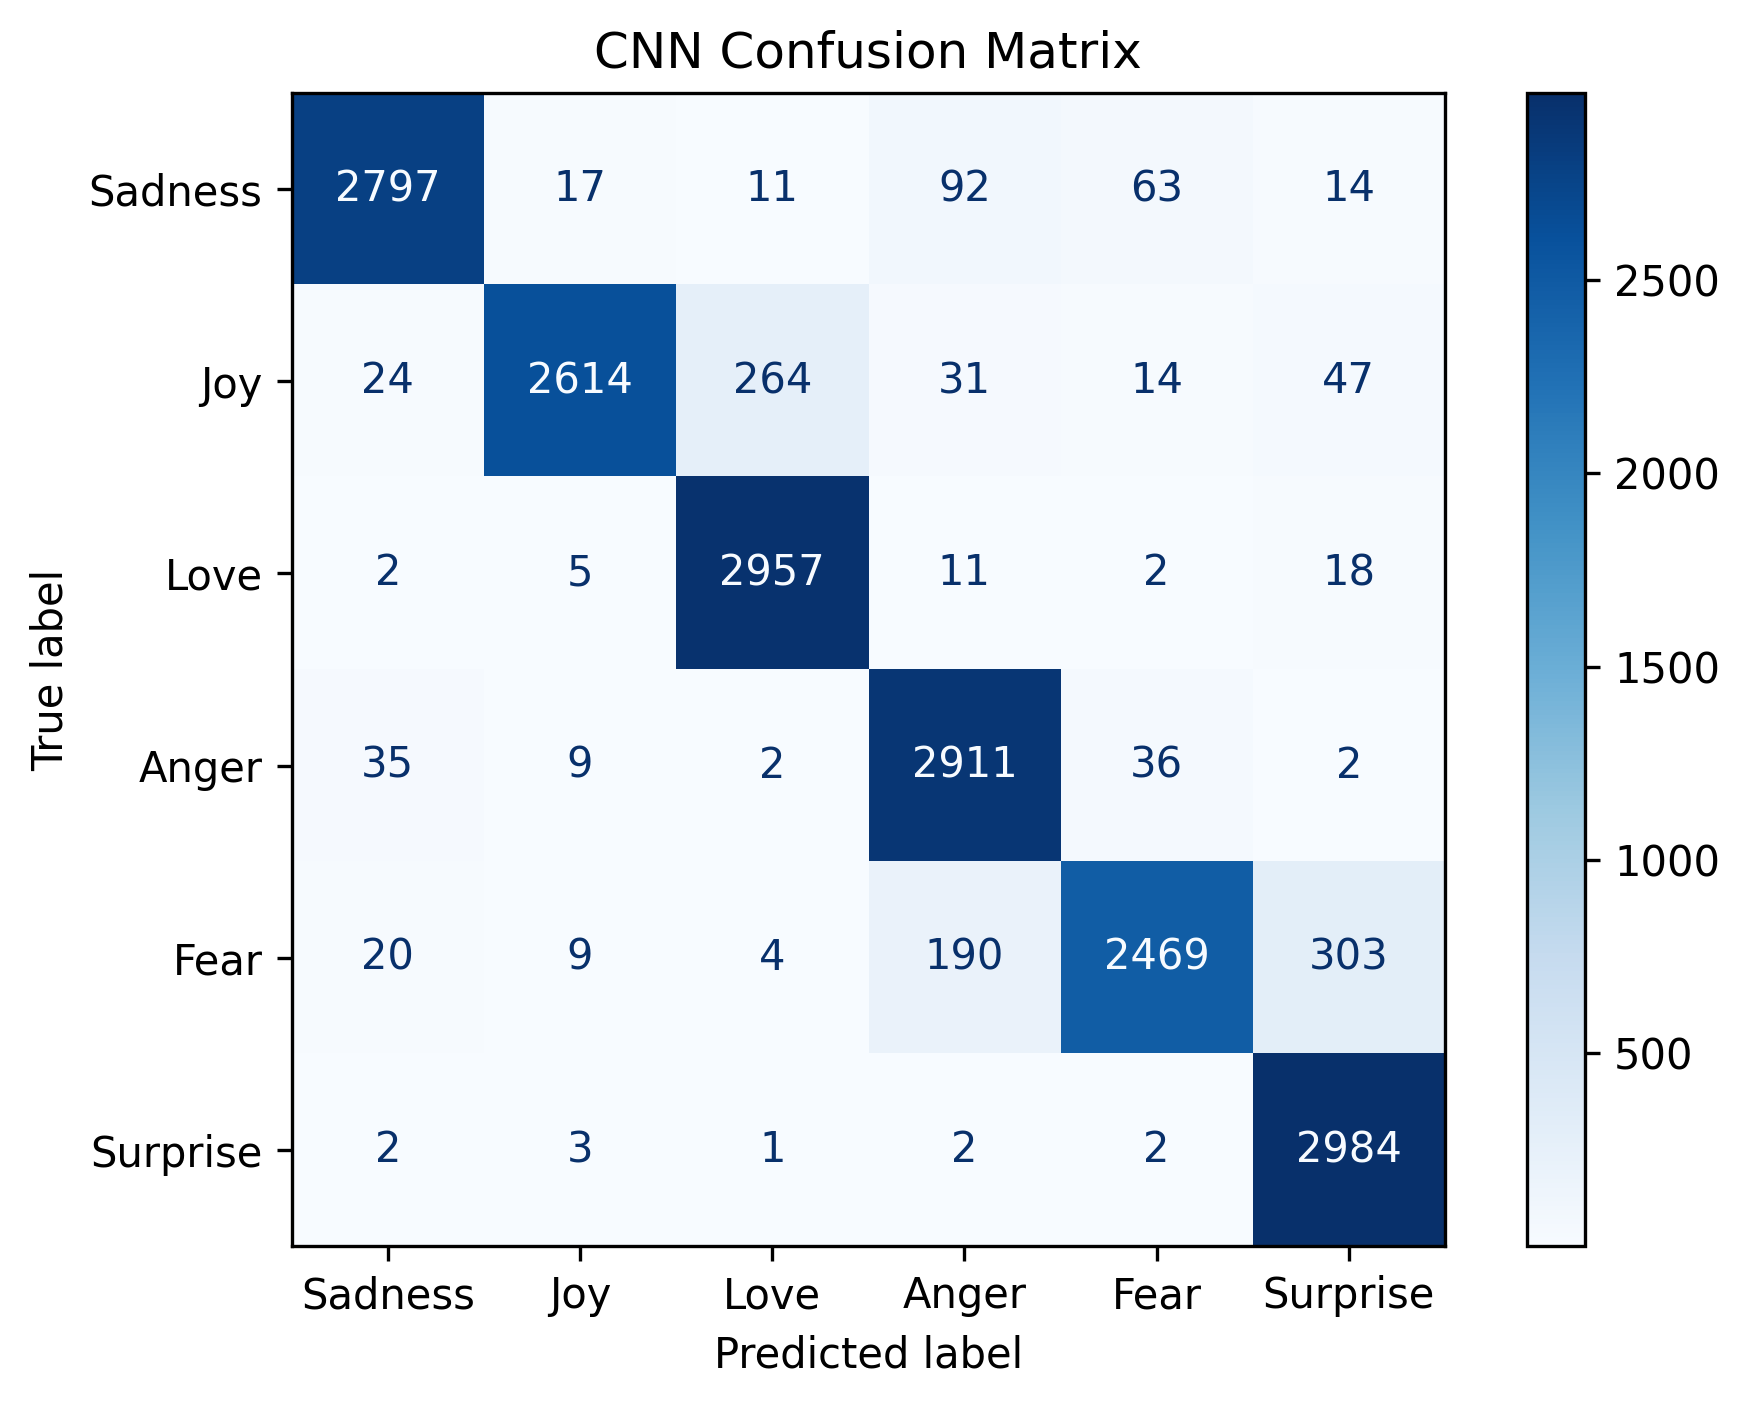
\includegraphics[width=0.48\linewidth]{figures/cnn_confusion_matrix.png}\\[4pt]
\makebox[0.48\linewidth]{\small (a) BiLSTM}\hfill\makebox[0.48\linewidth]{\small (b) CNN}\\[8pt]
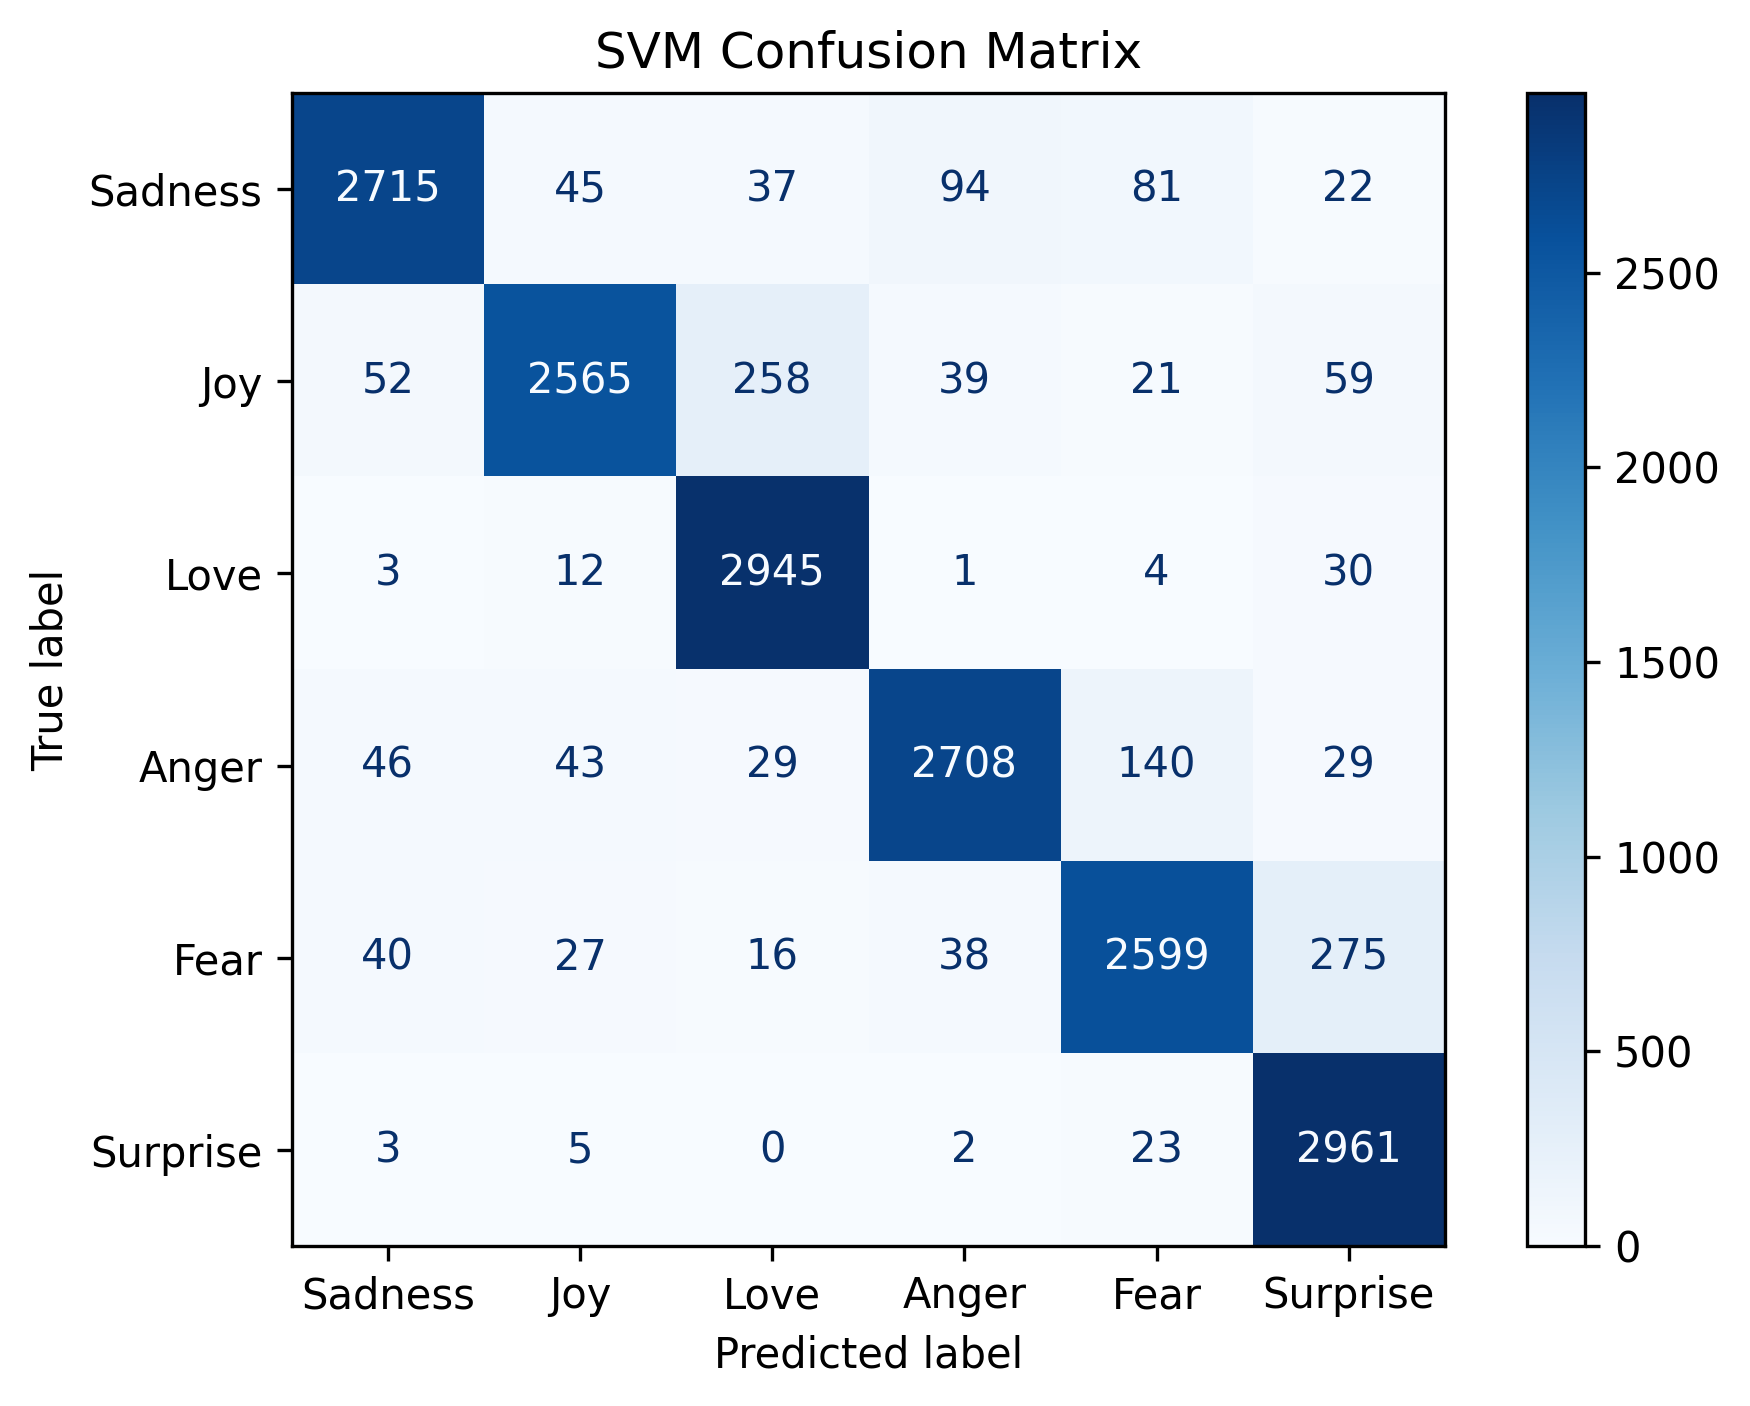
\includegraphics[width=0.48\linewidth]{figures/svm_confusion_matrix.png}\hfill
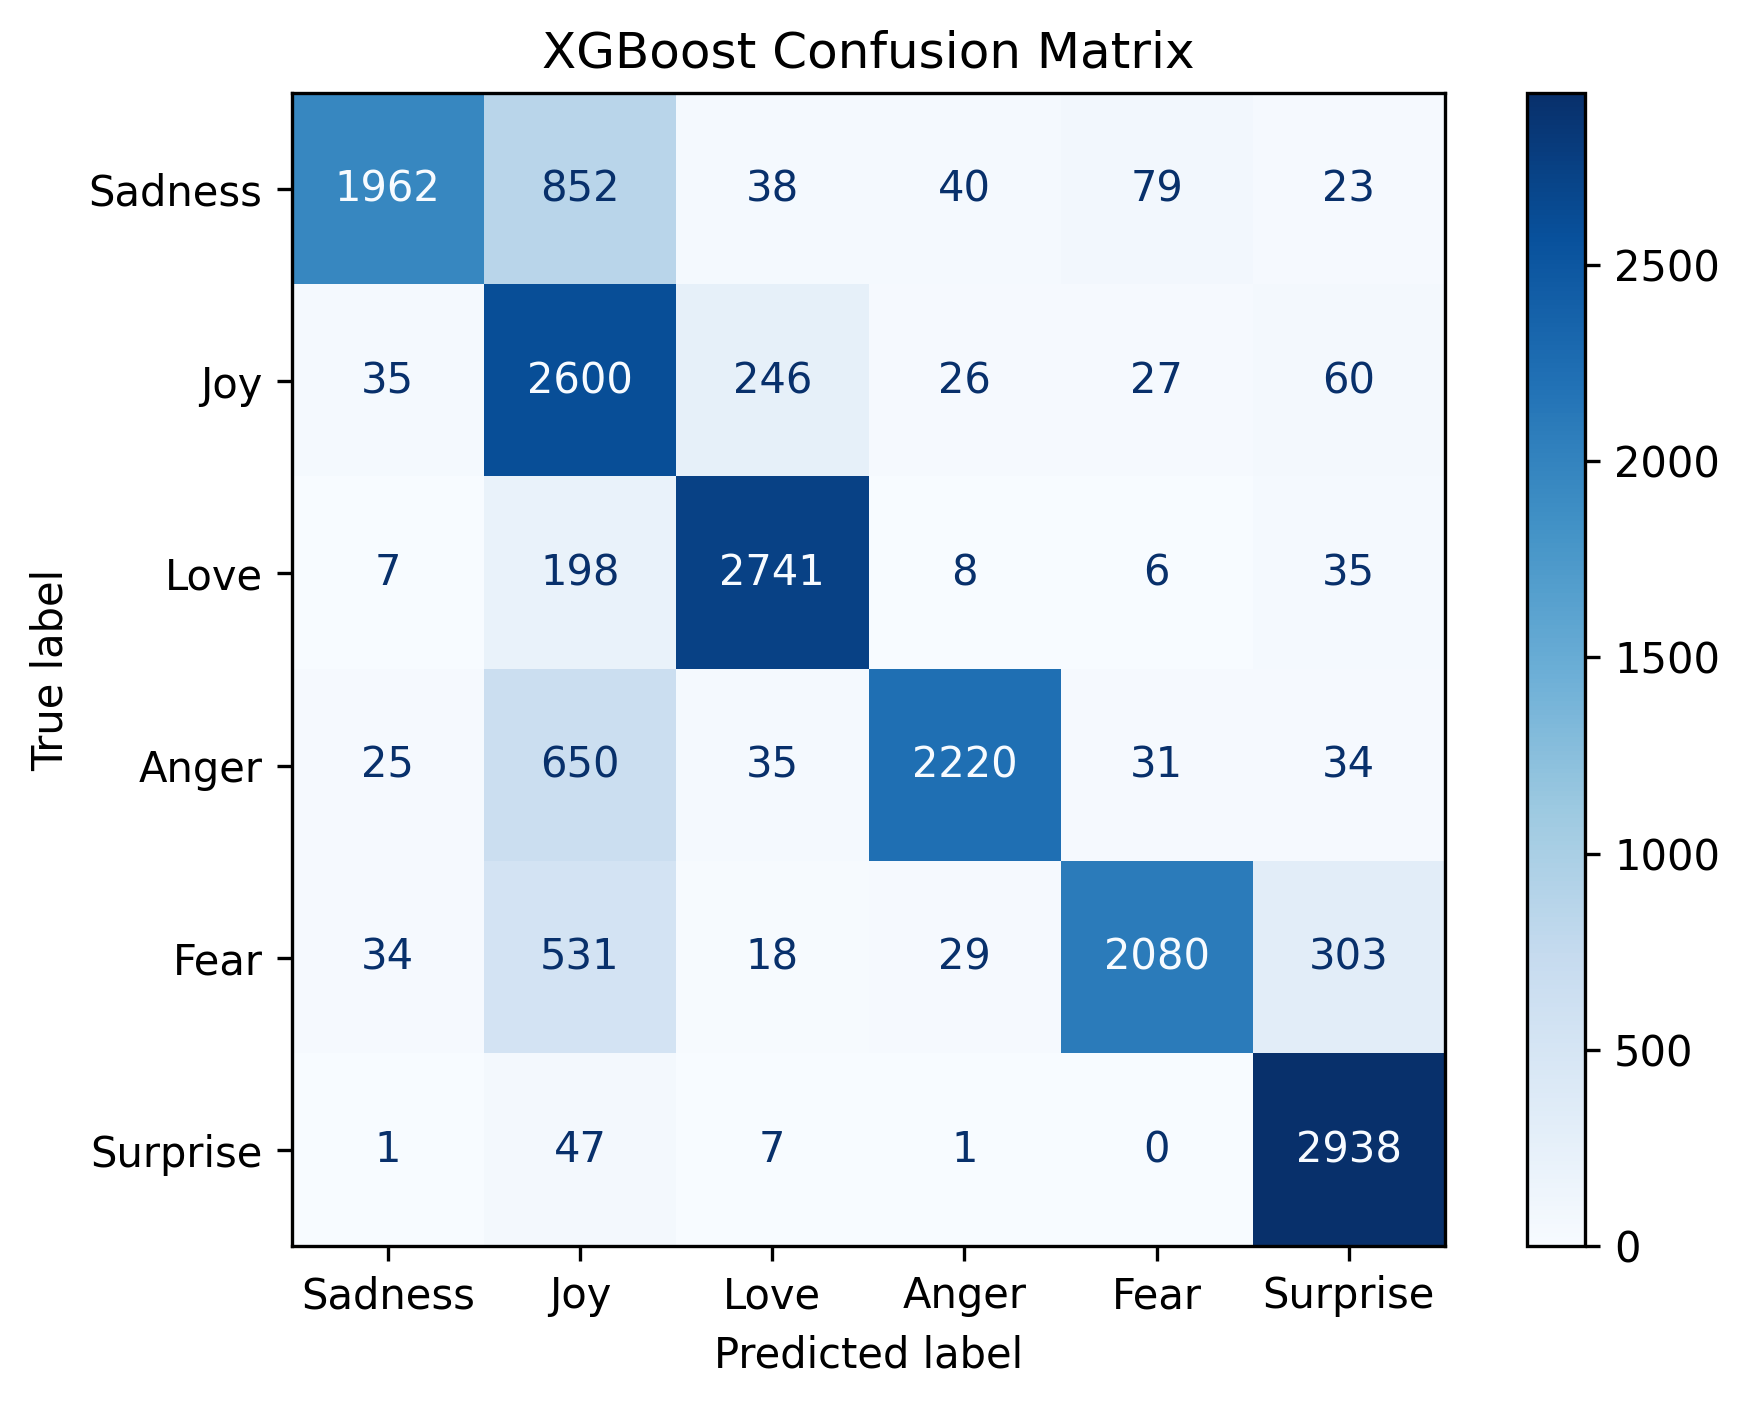
\includegraphics[width=0.48\linewidth]{figures/xgboost_confusion_matrix.png}\\[4pt]
\makebox[0.48\linewidth]{\small (c) SVM}\hfill\makebox[0.48\linewidth]{\small (d) XGBoost}
\caption{Confusion matrices for all four models on the balanced test set (17,967 samples). Joy$\leftrightarrow$Love and Fear$\rightarrow$Surprise misclassifications are consistent across architectures; XGBoost displays additional majority-class bias.}
\label{fig:confusion_matrices}
\end{figure}

%% ── A.2  EDA Distribution Plots ──
\needspace{12\baselineskip}
\subsection{Text Length and Word Count Distributions}

Figure~\ref{fig:text_length} shows (a)~a right-skewed text length distribution concentrated between 20--150 characters (median 86, mean 97.0), and (b)~per-class word count variation where Love produces the longest posts (median 19 words) and Sadness the shortest (median 16 words), informing the dynamic sequence padding strategy for DL models.

\begin{figure}[H]
\centering
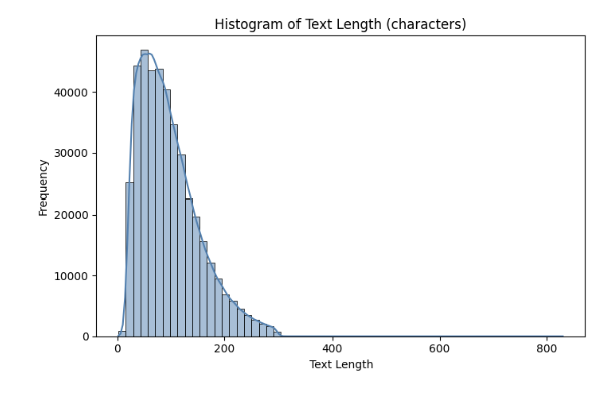
\includegraphics[width=0.48\linewidth]{figures/text_length_wordcount_1.png}\hfill
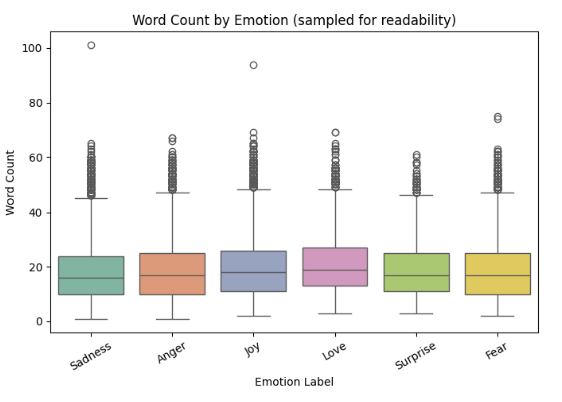
\includegraphics[width=0.48\linewidth]{figures/text_length_wordcount_2.png}\\[4pt]
\makebox[0.48\linewidth]{\small (a) Text length histogram}\hfill\makebox[0.48\linewidth]{\small (b) Word count by emotion class}
\caption{(a)~Text length distribution across the full 416,809-sample corpus. (b)~Word count boxplot by emotion class.}
\label{fig:text_length}
\label{fig:wordcount}
\end{figure}

Figure~\ref{fig:correlation_matrix} shows a Pearson correlation heatmap of the numeric features in the dataset. Text length and word count are near-perfectly correlated ($r=0.984$), while neither correlates with the encoded label ($r<0.03$), confirming that surface-level length statistics carry negligible class-discriminative signal.

\begin{figure}[H]
\centering
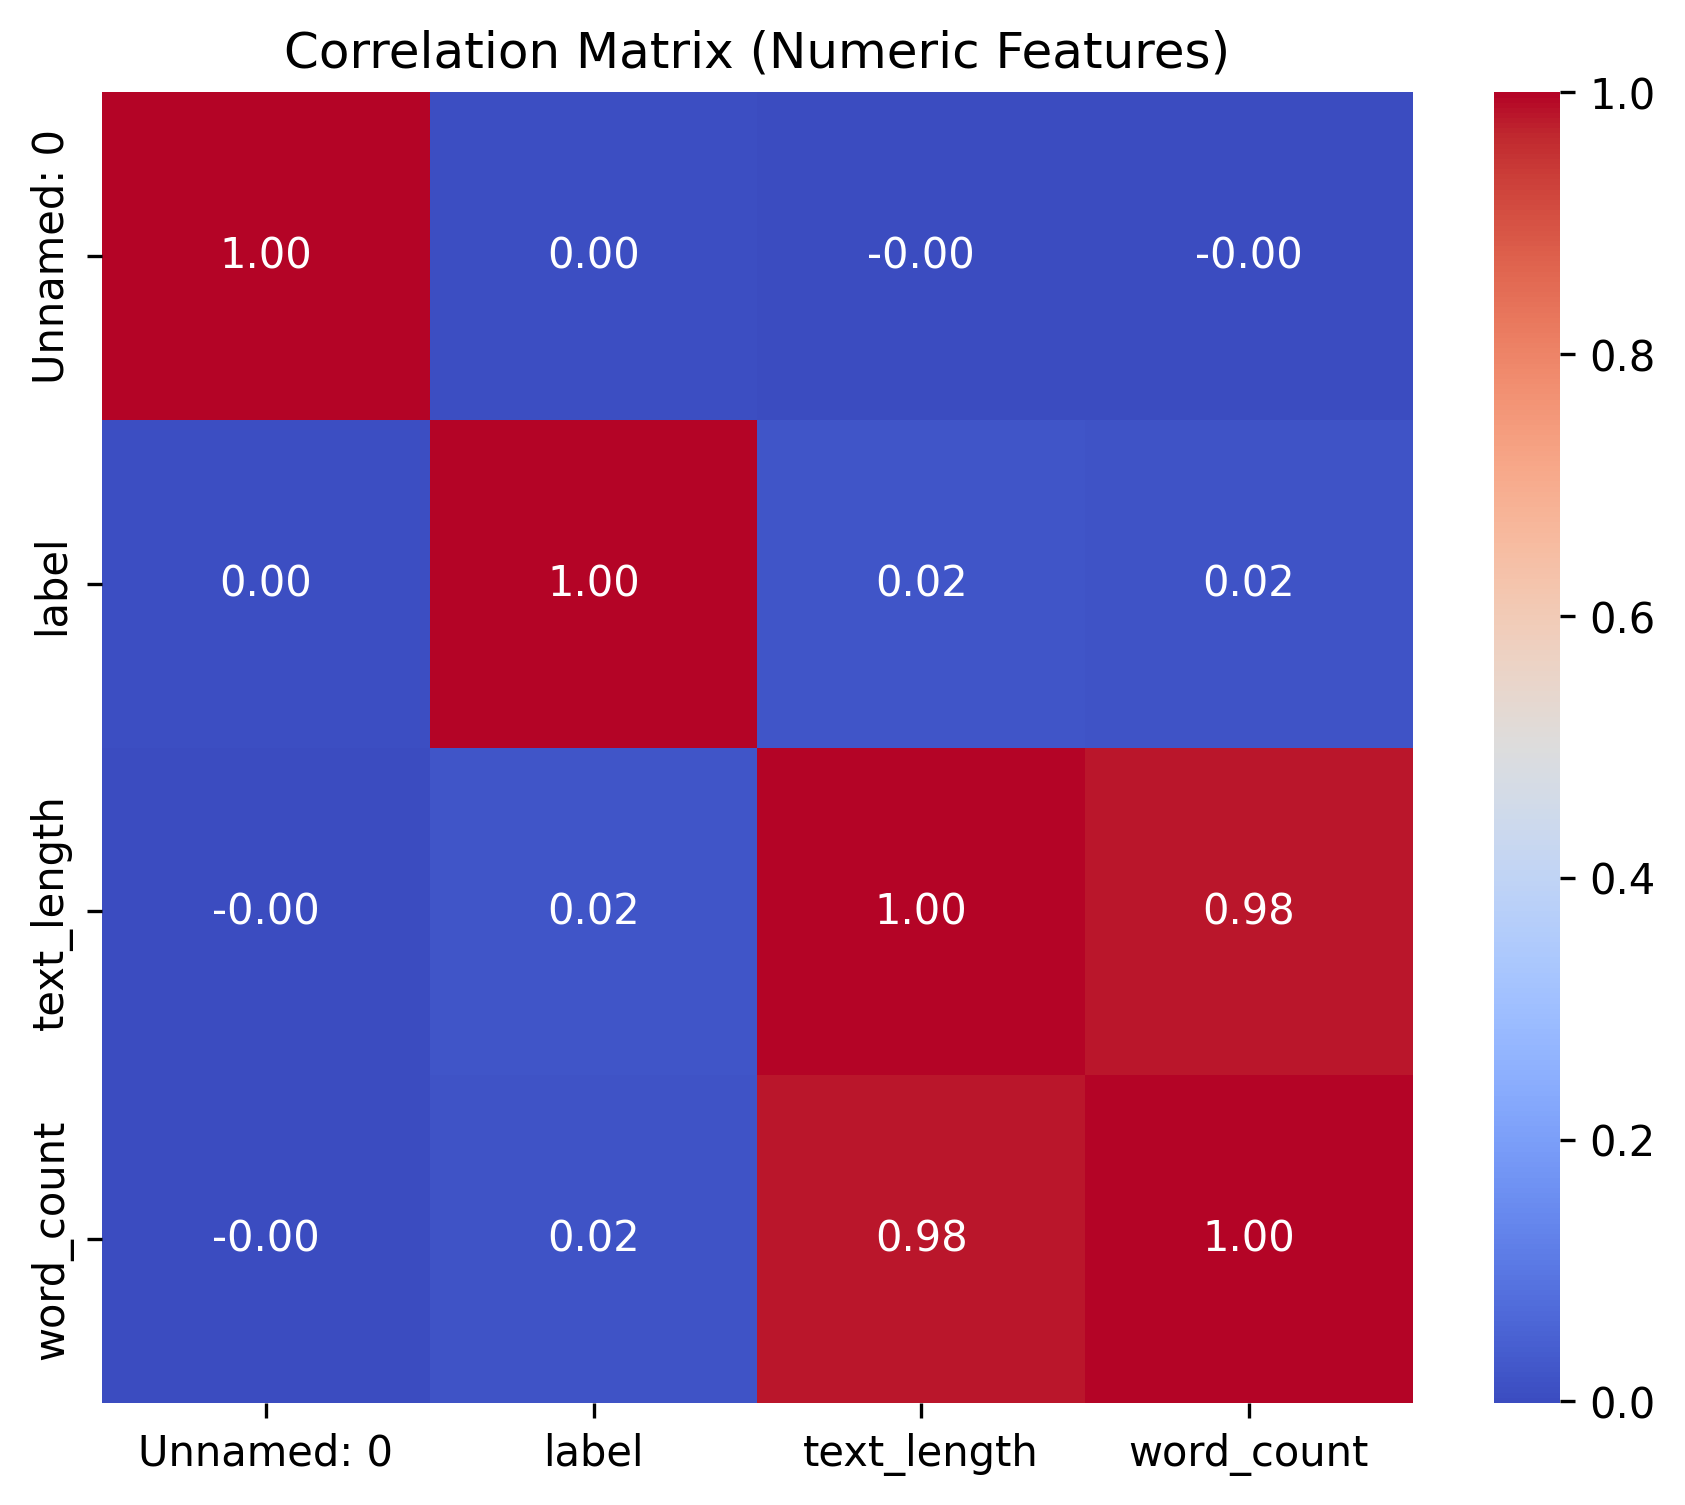
\includegraphics[width=0.55\linewidth]{figures/correlation_matrix.png}
\caption{Correlation matrix of numeric features. Text length and word count are highly correlated ($r=0.984$); neither correlates with the emotion label.}
\label{fig:correlation_matrix}
\end{figure}

%% ── A.3  Process Flow ──
\clearpage
\subsection{Process Flow Diagram}

Figure~\ref{fig:process_flow} presents an alternative view of the pipeline architecture (Figure~\ref{fig:pipeline}), showing each stage in detail: data ingestion, preprocessing, parallel ML/DL feature extraction, model training, evaluation, and deployment.

\begin{figure}[H]
\centering
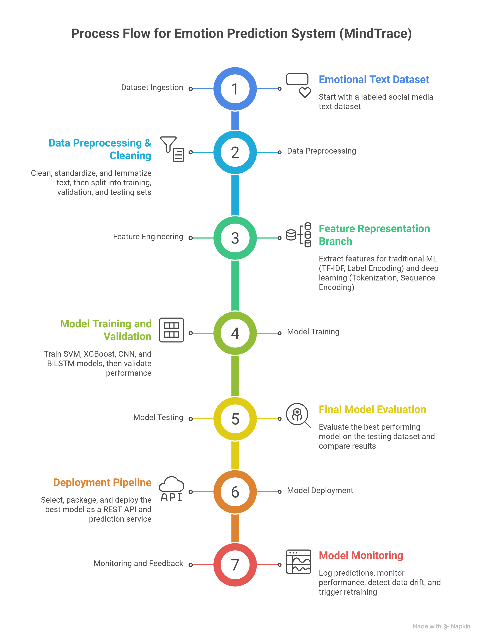
\includegraphics[width=0.65\linewidth]{figures/process_flow.png}
\caption{MindTrace detailed process flow --- from raw dataset through preprocessing, feature extraction, model training, evaluation, and deployment.}
\label{fig:process_flow}
\end{figure}

%% ── A.4  Word Clouds ──
\needspace{20\baselineskip}
\subsection{Per-Class Word Clouds}

Figure~\ref{fig:wordclouds} highlights the most frequent tokens per emotion after preprocessing. Joy and Love share positively-valenced tokens (``happy'', ``love'', ``good''), explaining the Joy$\leftrightarrow$Love confusion. Fear and Surprise share high-arousal tokens (``suddenly'', ``shocked''), corroborating the Fear$\rightarrow$Surprise pattern. Anger displays uniquely aggressive vocabulary (``hate'', ``angry''), making it the most separable class.

\begin{figure}[H]
\centering

\includegraphics[width=0.46\linewidth]{figures/wordcloud_anger.png}\hfill

\includegraphics[width=0.46\linewidth]{figures/wordcloud_fear.png}\\[4pt]
\makebox[0.46\linewidth]{\small (a) Anger}\hfill\makebox[0.46\linewidth]{\small (b) Fear}\\[8pt]

\includegraphics[width=0.46\linewidth]{figures/wordcloud_joy.png}\hfill

\includegraphics[width=0.46\linewidth]{figures/wordcloud_love.png}\\[4pt]
\makebox[0.46\linewidth]{\small (c) Joy}\hfill\makebox[0.46\linewidth]{\small (d) Love}\\[8pt]

\includegraphics[width=0.46\linewidth]{figures/wordcloud_sadness.png}\hfill

\includegraphics[width=0.46\linewidth]{figures/wordcloud_surprise.png}\\[4pt]
\makebox[0.46\linewidth]{\small (e) Sadness}\hfill\makebox[0.46\linewidth]{\small (f) Surprise}
\caption{Per-class word clouds from the preprocessed corpus. Joy and Love share positive vocabulary; Fear and Surprise share high-arousal tokens.}
\label{fig:wordclouds}
\end{figure}

%% ── A.5  Web Application Interface ──
\needspace{10\baselineskip}
\subsection{Web Application Interface}
\label{sec:app_ui}

The deployed MindTrace web application provides four main views: a Predict tab for real-time emotion classification, a Dashboard tab for model performance analytics, a History tab displaying the session prediction log with per-emotion summary chips and a clear-all function, and an About tab summarising the research methodology.

\needspace{8\baselineskip}
\subsubsection{Predict Tab}

Figure~\ref{fig:ui_overview} shows the default Predict tab and an Anger prediction at 98.0\% confidence. The preprocessing trace demonstrates retention of the negation word ``never'' during stopword removal. Figure~\ref{fig:ui_love}(a,\,b) shows Love (98.8\%) and Sadness (99.8\%) predictions; the Love example confirms the known Joy$\leftrightarrow$Love overlap pattern, with Joy as the nearest competitor at 1.2\%.

\begin{figure}[H]
\centering

\includegraphics[width=0.48\linewidth]{img/overview.png}\hfill

\includegraphics[width=0.48\linewidth]{img/Anger.png}\\[4pt]
\makebox[0.48\linewidth]{\small (a) Default state}\hfill\makebox[0.48\linewidth]{\small (b) Anger --- 98.0\% confidence}
\caption{Predict tab --- (a)~default state with example sentences; (b)~Anger detected at 98.0\% confidence with preprocessing trace.}
\label{fig:ui_overview}
\label{fig:ui_anger}
\end{figure}

\begin{figure}[H]
\centering
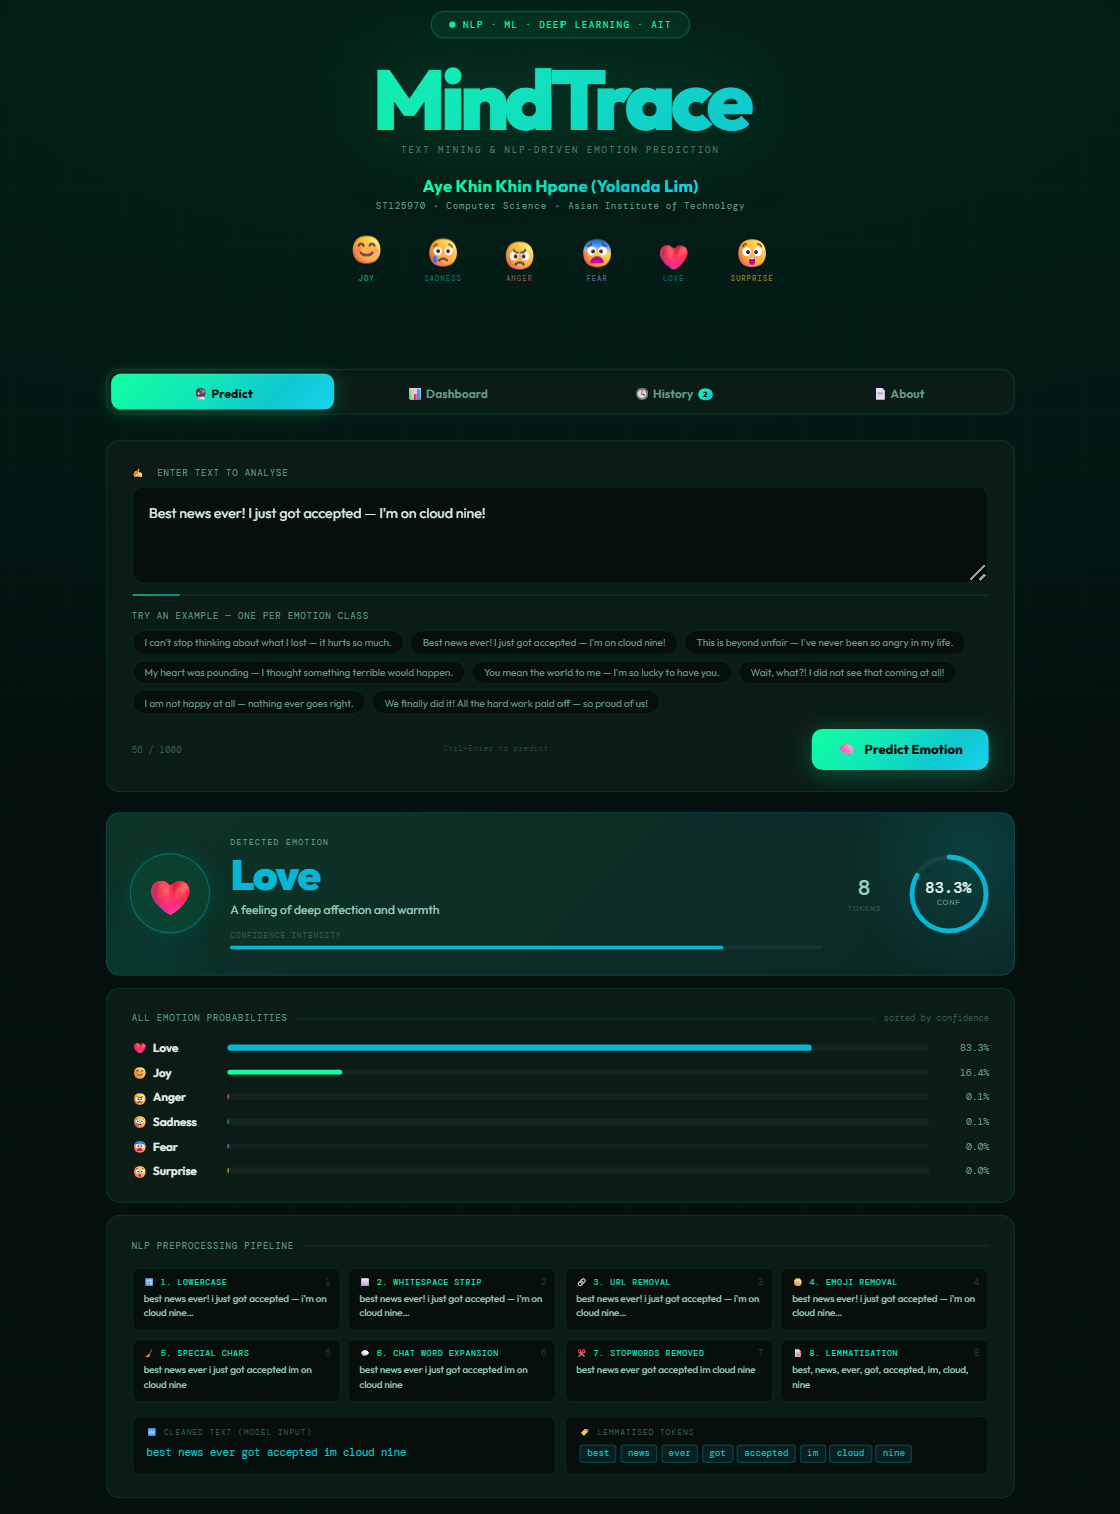
\includegraphics[width=0.48\linewidth]{img/love.png}\hfill
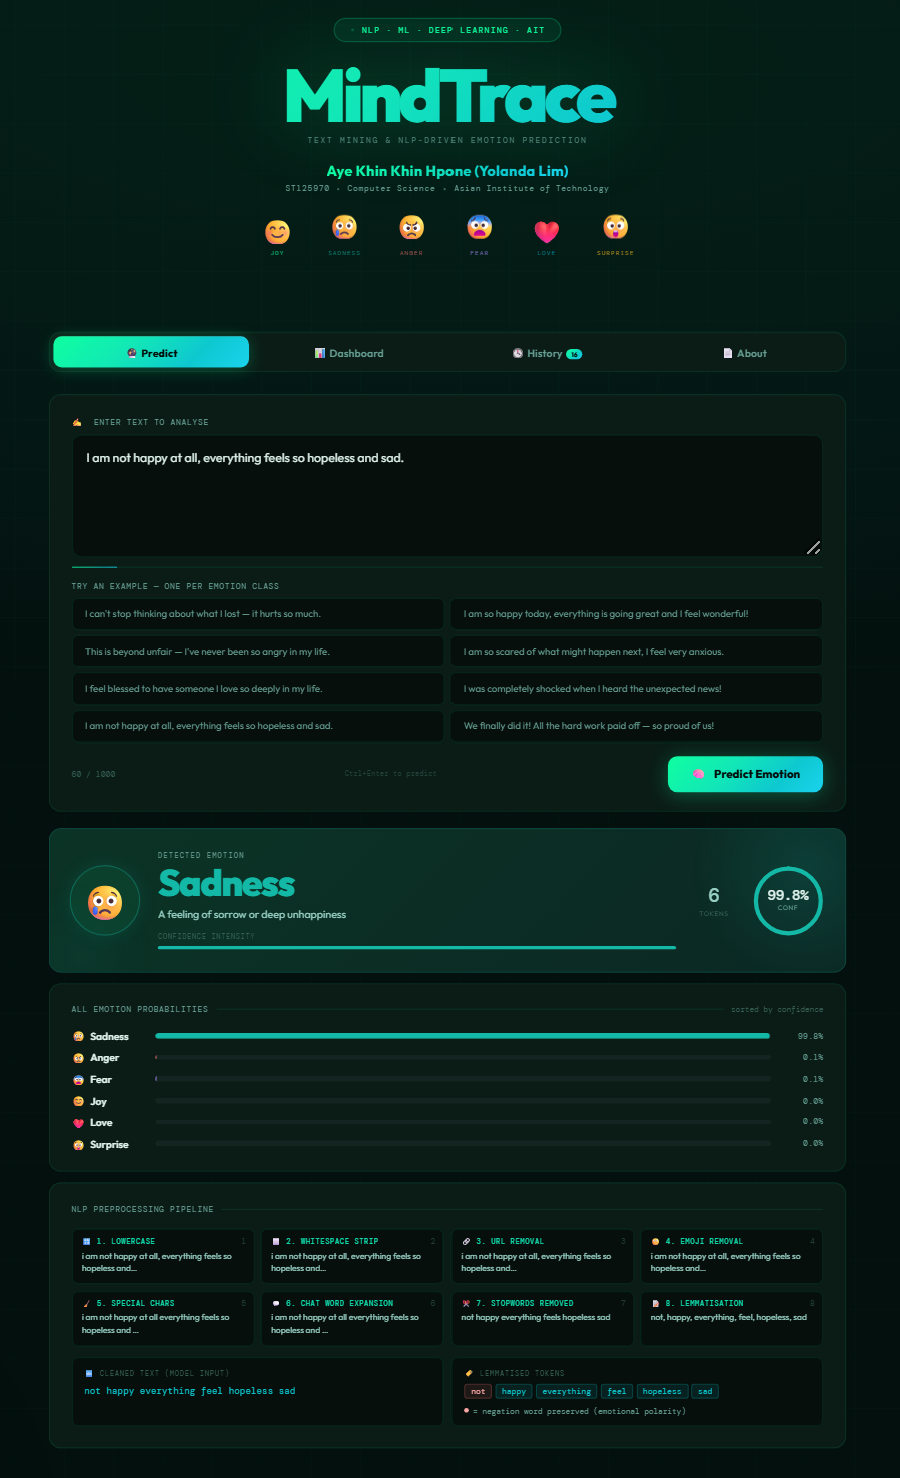
\includegraphics[width=0.48\linewidth]{img/sadness.png}\\[4pt]
\makebox[0.48\linewidth]{\small (a) Love --- 98.8\% confidence}\hfill\makebox[0.48\linewidth]{\small (b) Sadness --- 99.8\% confidence}
\caption{Predict tab --- (a)~Love detected at 98.8\% confidence (Joy runner-up at 1.2\%); (b)~Sadness detected at 99.8\% confidence.}
\label{fig:ui_love}
\label{fig:ui_sadness}
\end{figure}

\needspace{8\baselineskip}
\subsubsection{Dashboard Tab}

Figure~\ref{fig:ui_dashboard} presents the model performance dashboard with accuracy/precision/recall/F1 comparison across all four models, detailed results table, radar chart, class distribution, confusion pair analysis, and training curves.

\begin{figure}[H]
\centering
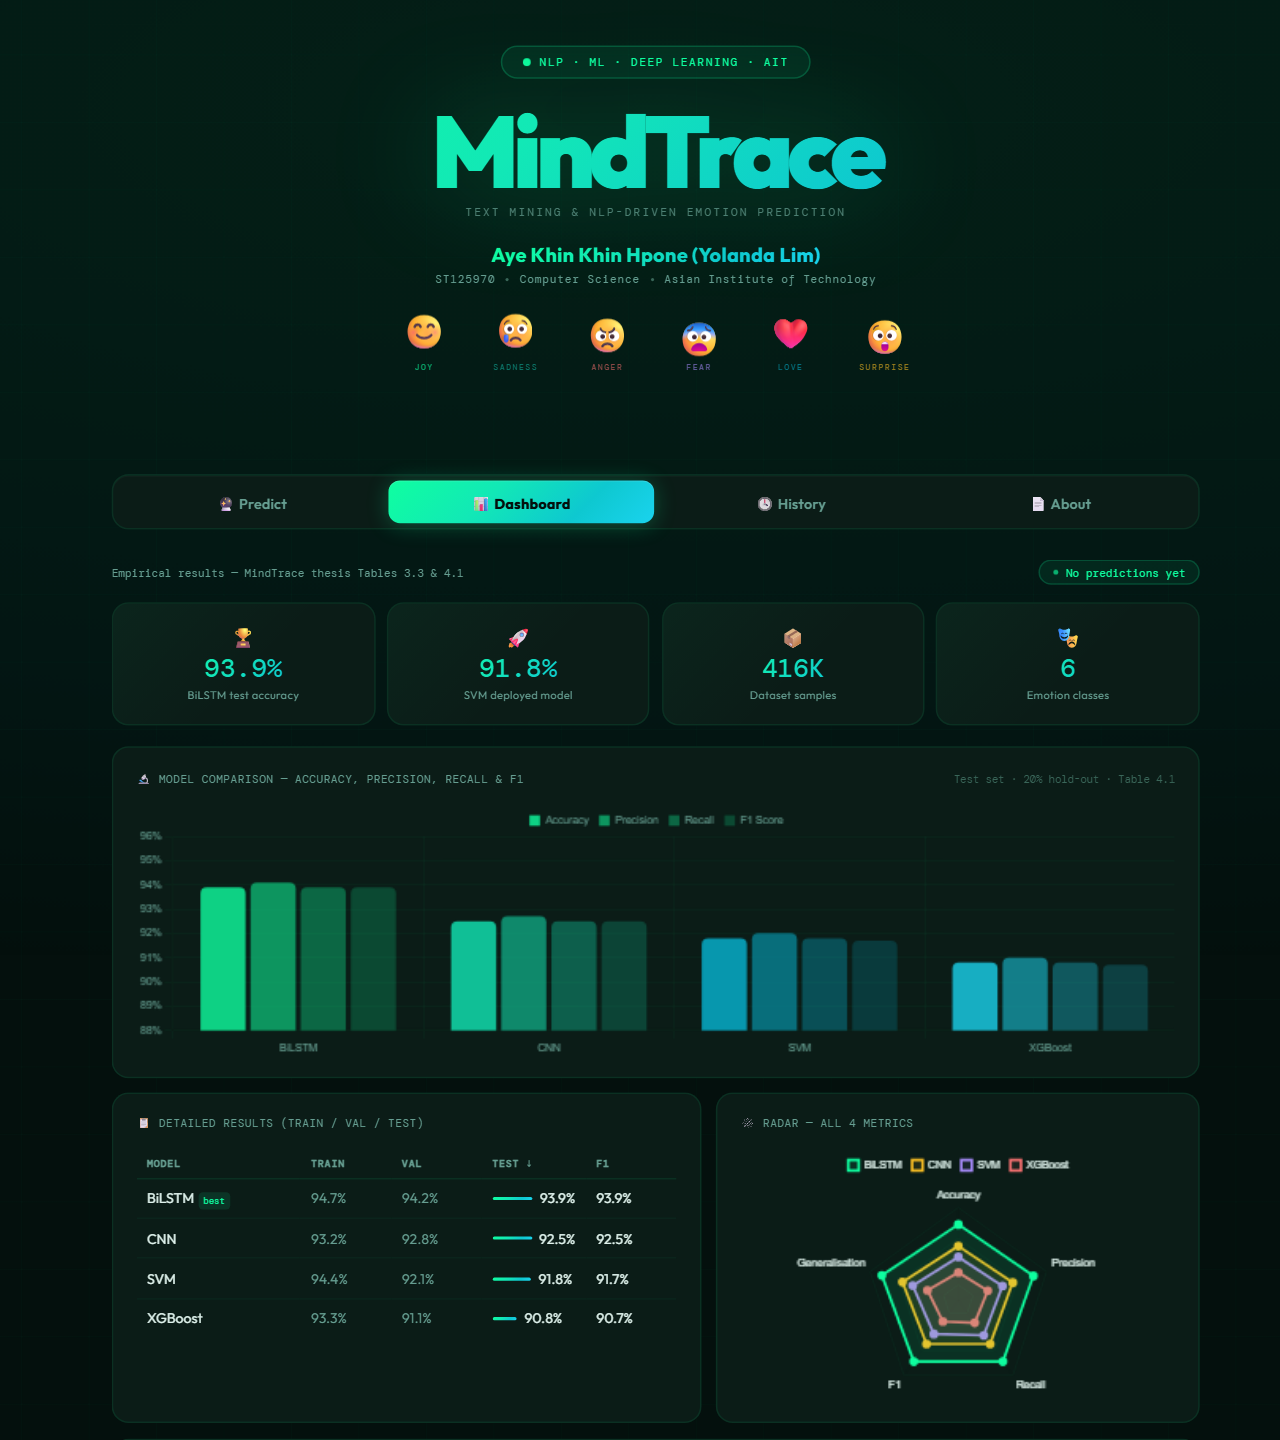
\includegraphics[width=0.48\linewidth]{img/dashboard.png}\hfill
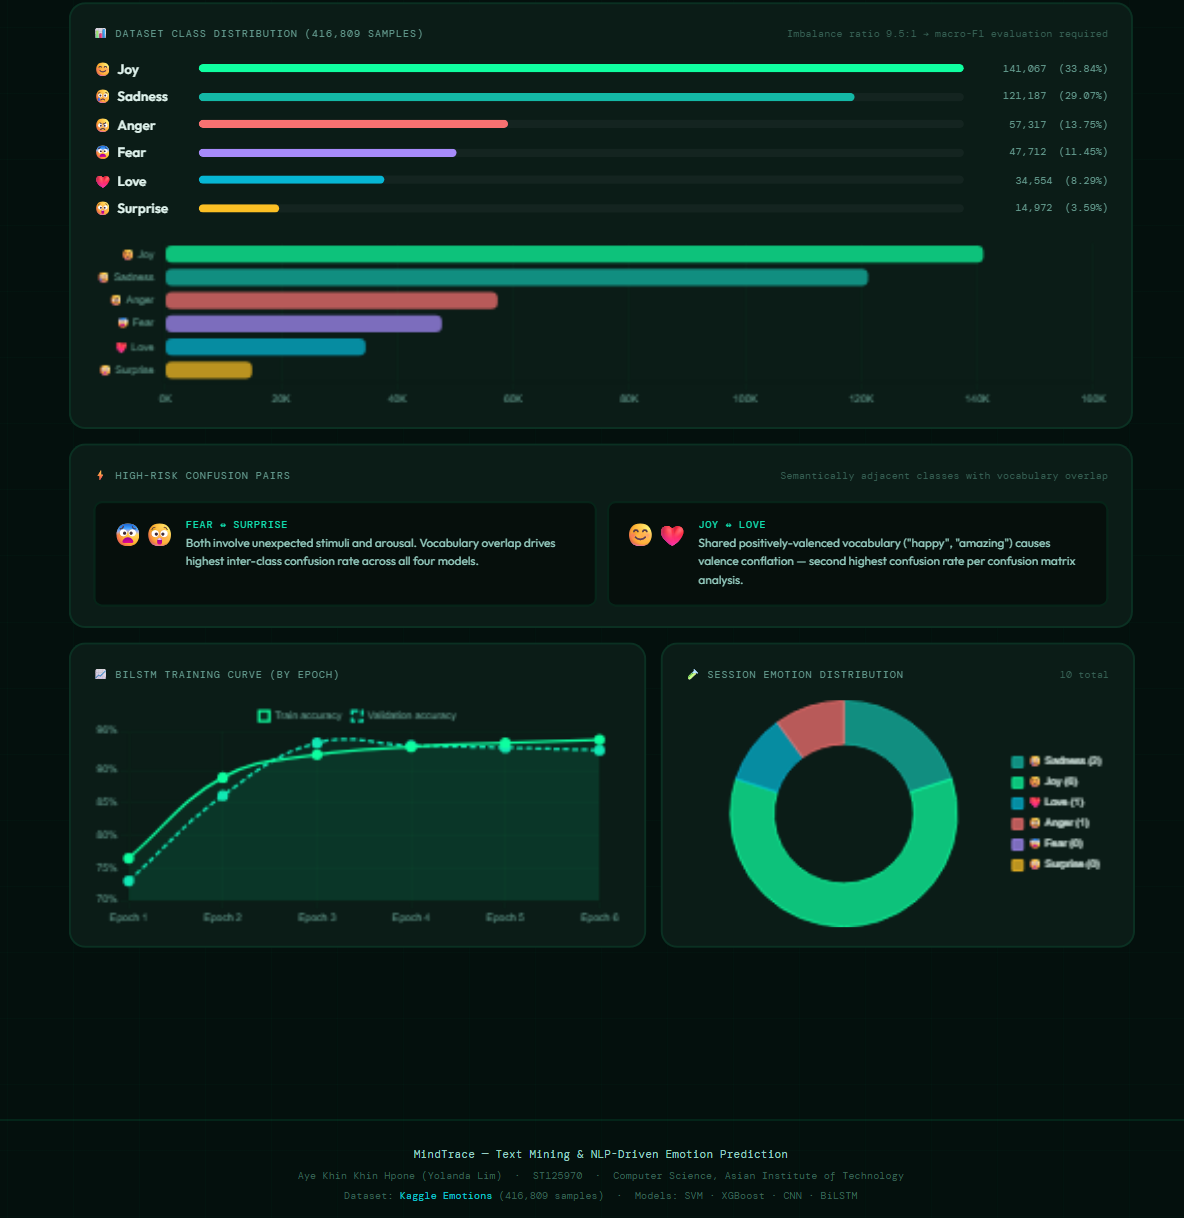
\includegraphics[width=0.48\linewidth]{img/dashboard_2.png}\\[4pt]
\makebox[0.48\linewidth]{\small (a) Upper section}\hfill\makebox[0.48\linewidth]{\small (b) Lower section}
\caption{Dashboard tab --- (a)~summary statistics, model comparison bar chart, results table, and radar chart; (b)~class distribution, high-risk confusion pairs, and BiLSTM training curves.}
\label{fig:ui_dashboard}
\label{fig:ui_dashboard2}
\end{figure}

\clearpage
\subsubsection{About Tab}

Figure~\ref{fig:ui_about} presents the About page summarising the research question, dataset, NLP pipeline, model architectures, EDA findings, and contributions.

\begin{figure}[H]
\centering

\includegraphics[width=0.7\linewidth]{img/Aboutsection_whole.png}
\caption{About tab --- full-page view summarising the research methodology, dataset, models, EDA findings, and contributions.}
\label{fig:ui_about}
\end{figure}

%% ── A.6  Ablation Study Visualisations ──
\clearpage
\subsection{Ablation Study Visualisations}
\label{sec:ablation_viz}

Figures~\ref{fig:ablation_svm_f1} and~\ref{fig:ablation_bilstm_f1} complement the tabular ablation results in Section~\ref{sec:ablation}. Dashed lines indicate the baseline (full-pipeline) score; bars that fall below the line quantify each preprocessing step's contribution.

\begin{figure}[H]
\centering
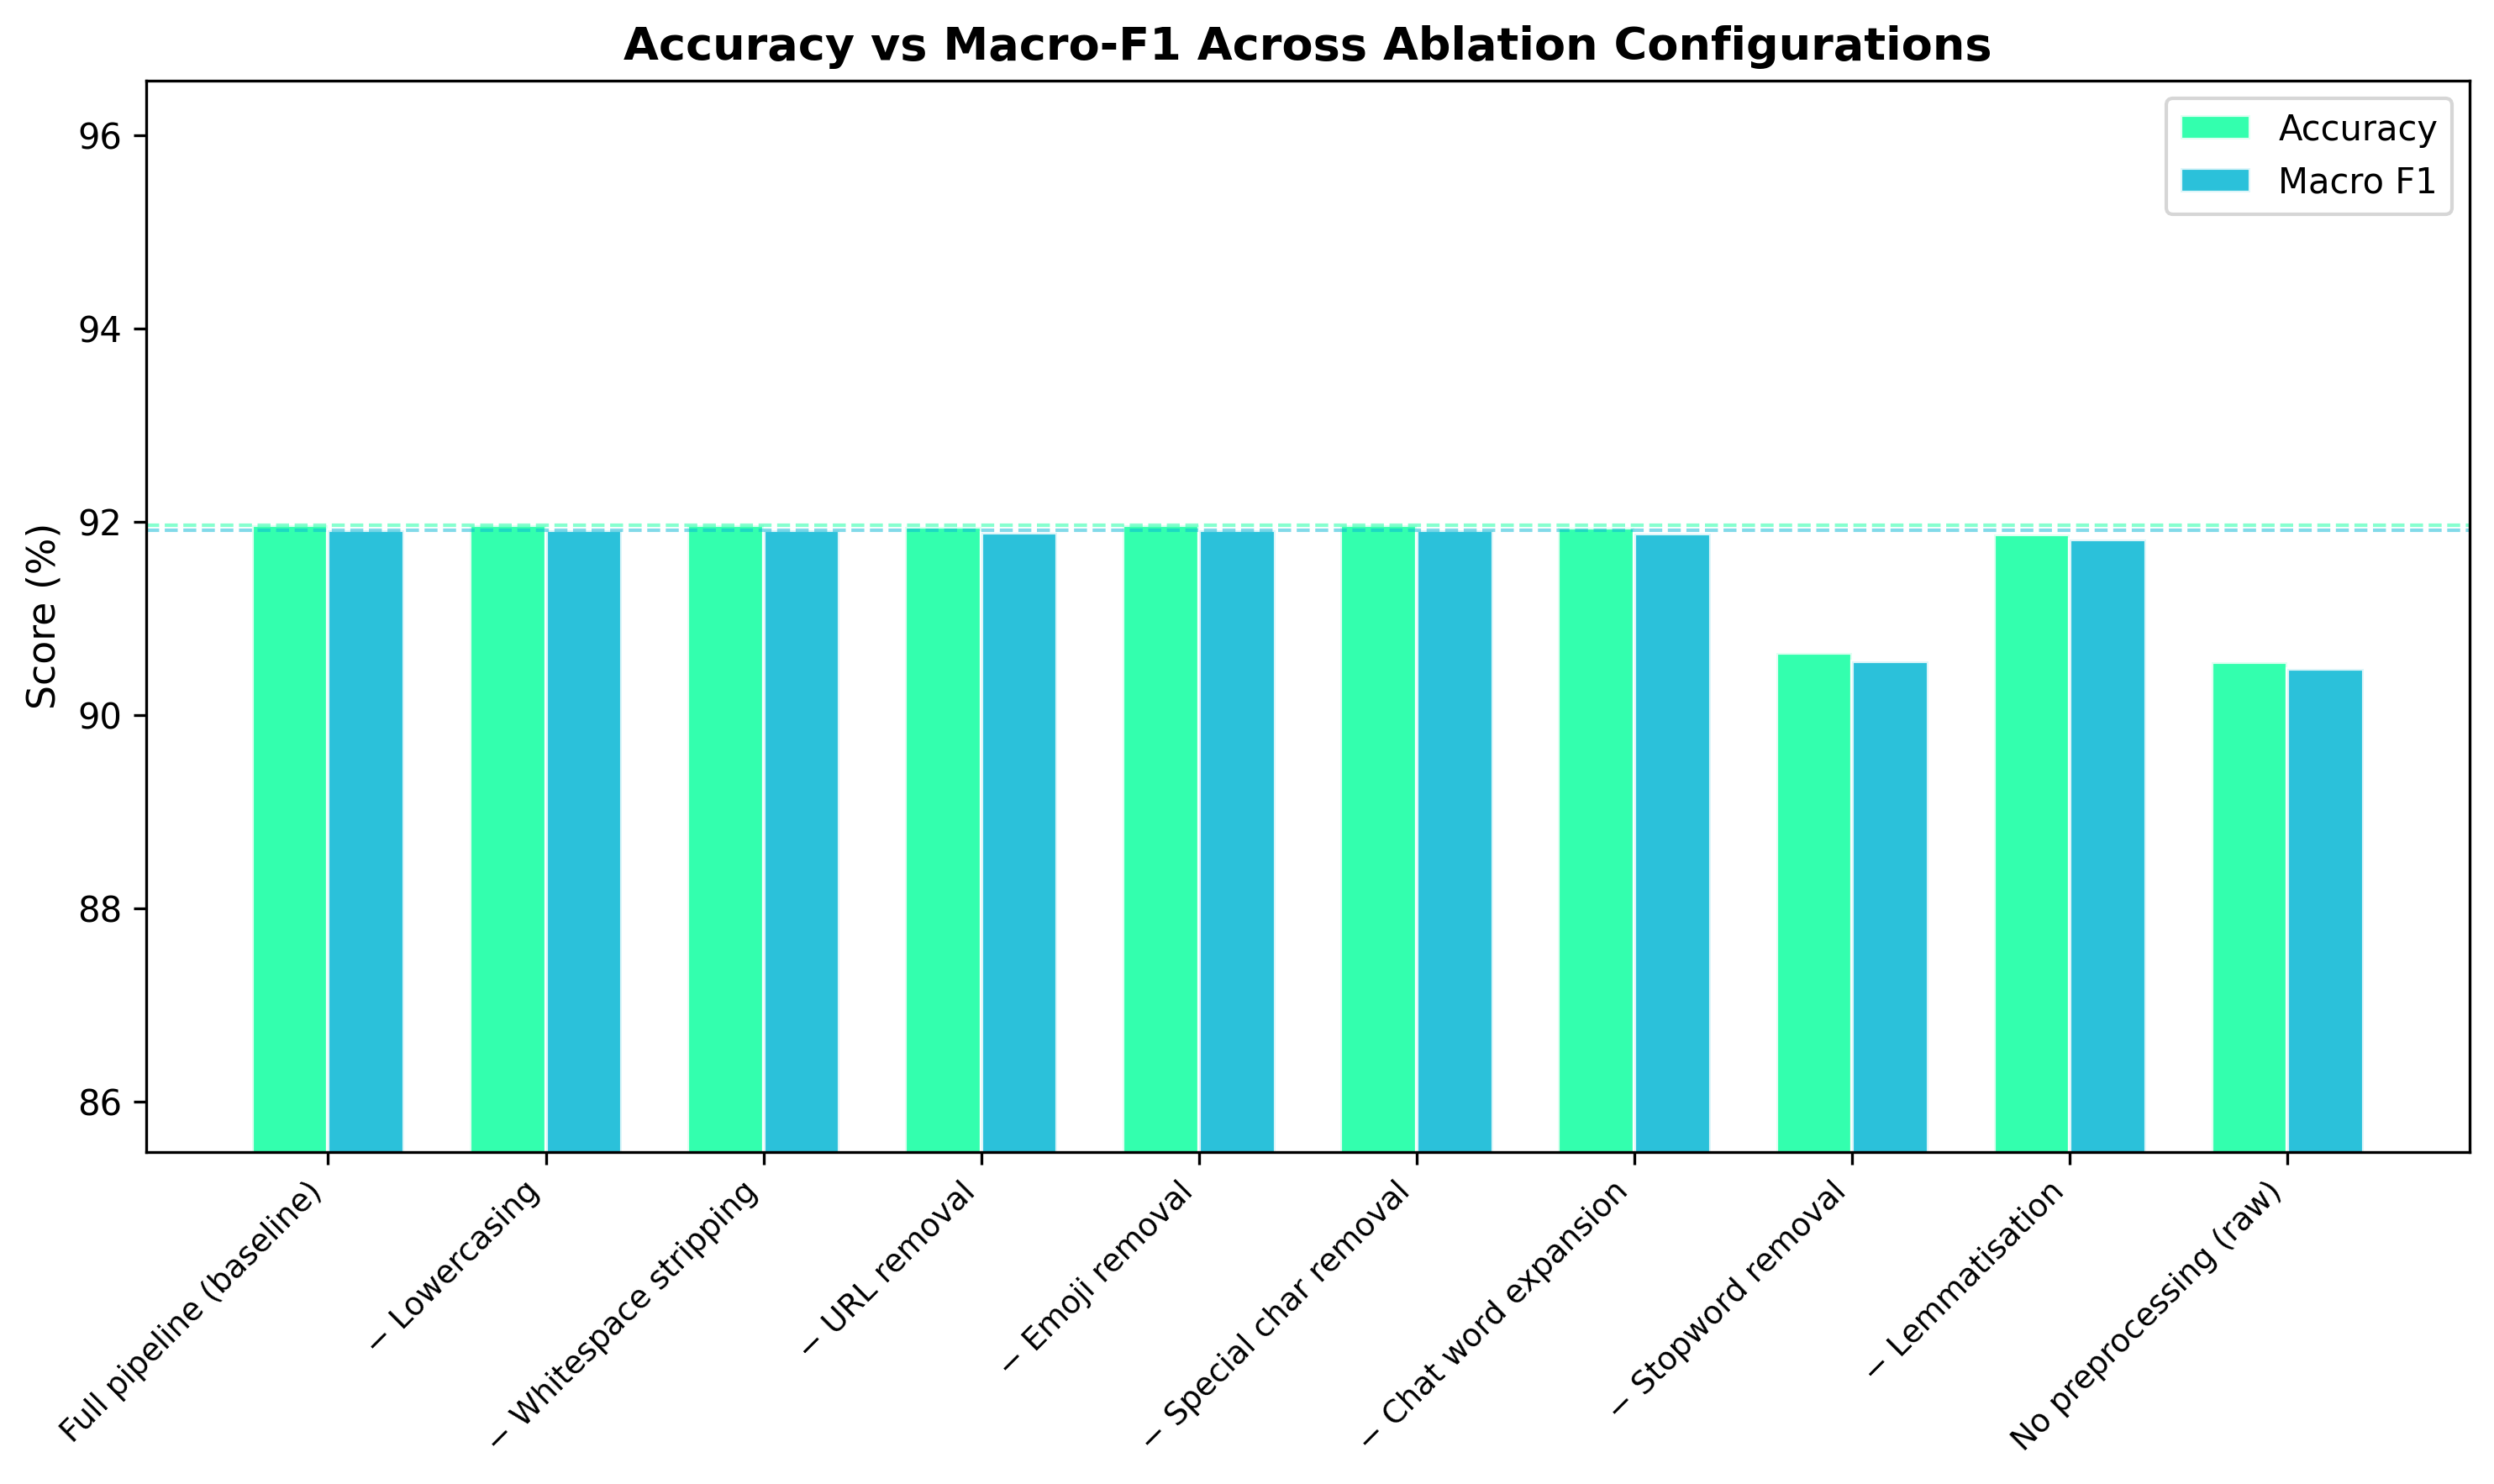
\includegraphics[width=0.85\linewidth]{figures/ablation_study_f1.png}
\caption{SVM ablation --- Accuracy and Macro-F1 across preprocessing configurations. Stopword removal and the no-preprocessing control show the largest drops from the full-pipeline baseline.}
\label{fig:ablation_svm_f1}
\end{figure}

\begin{figure}[H]
\centering
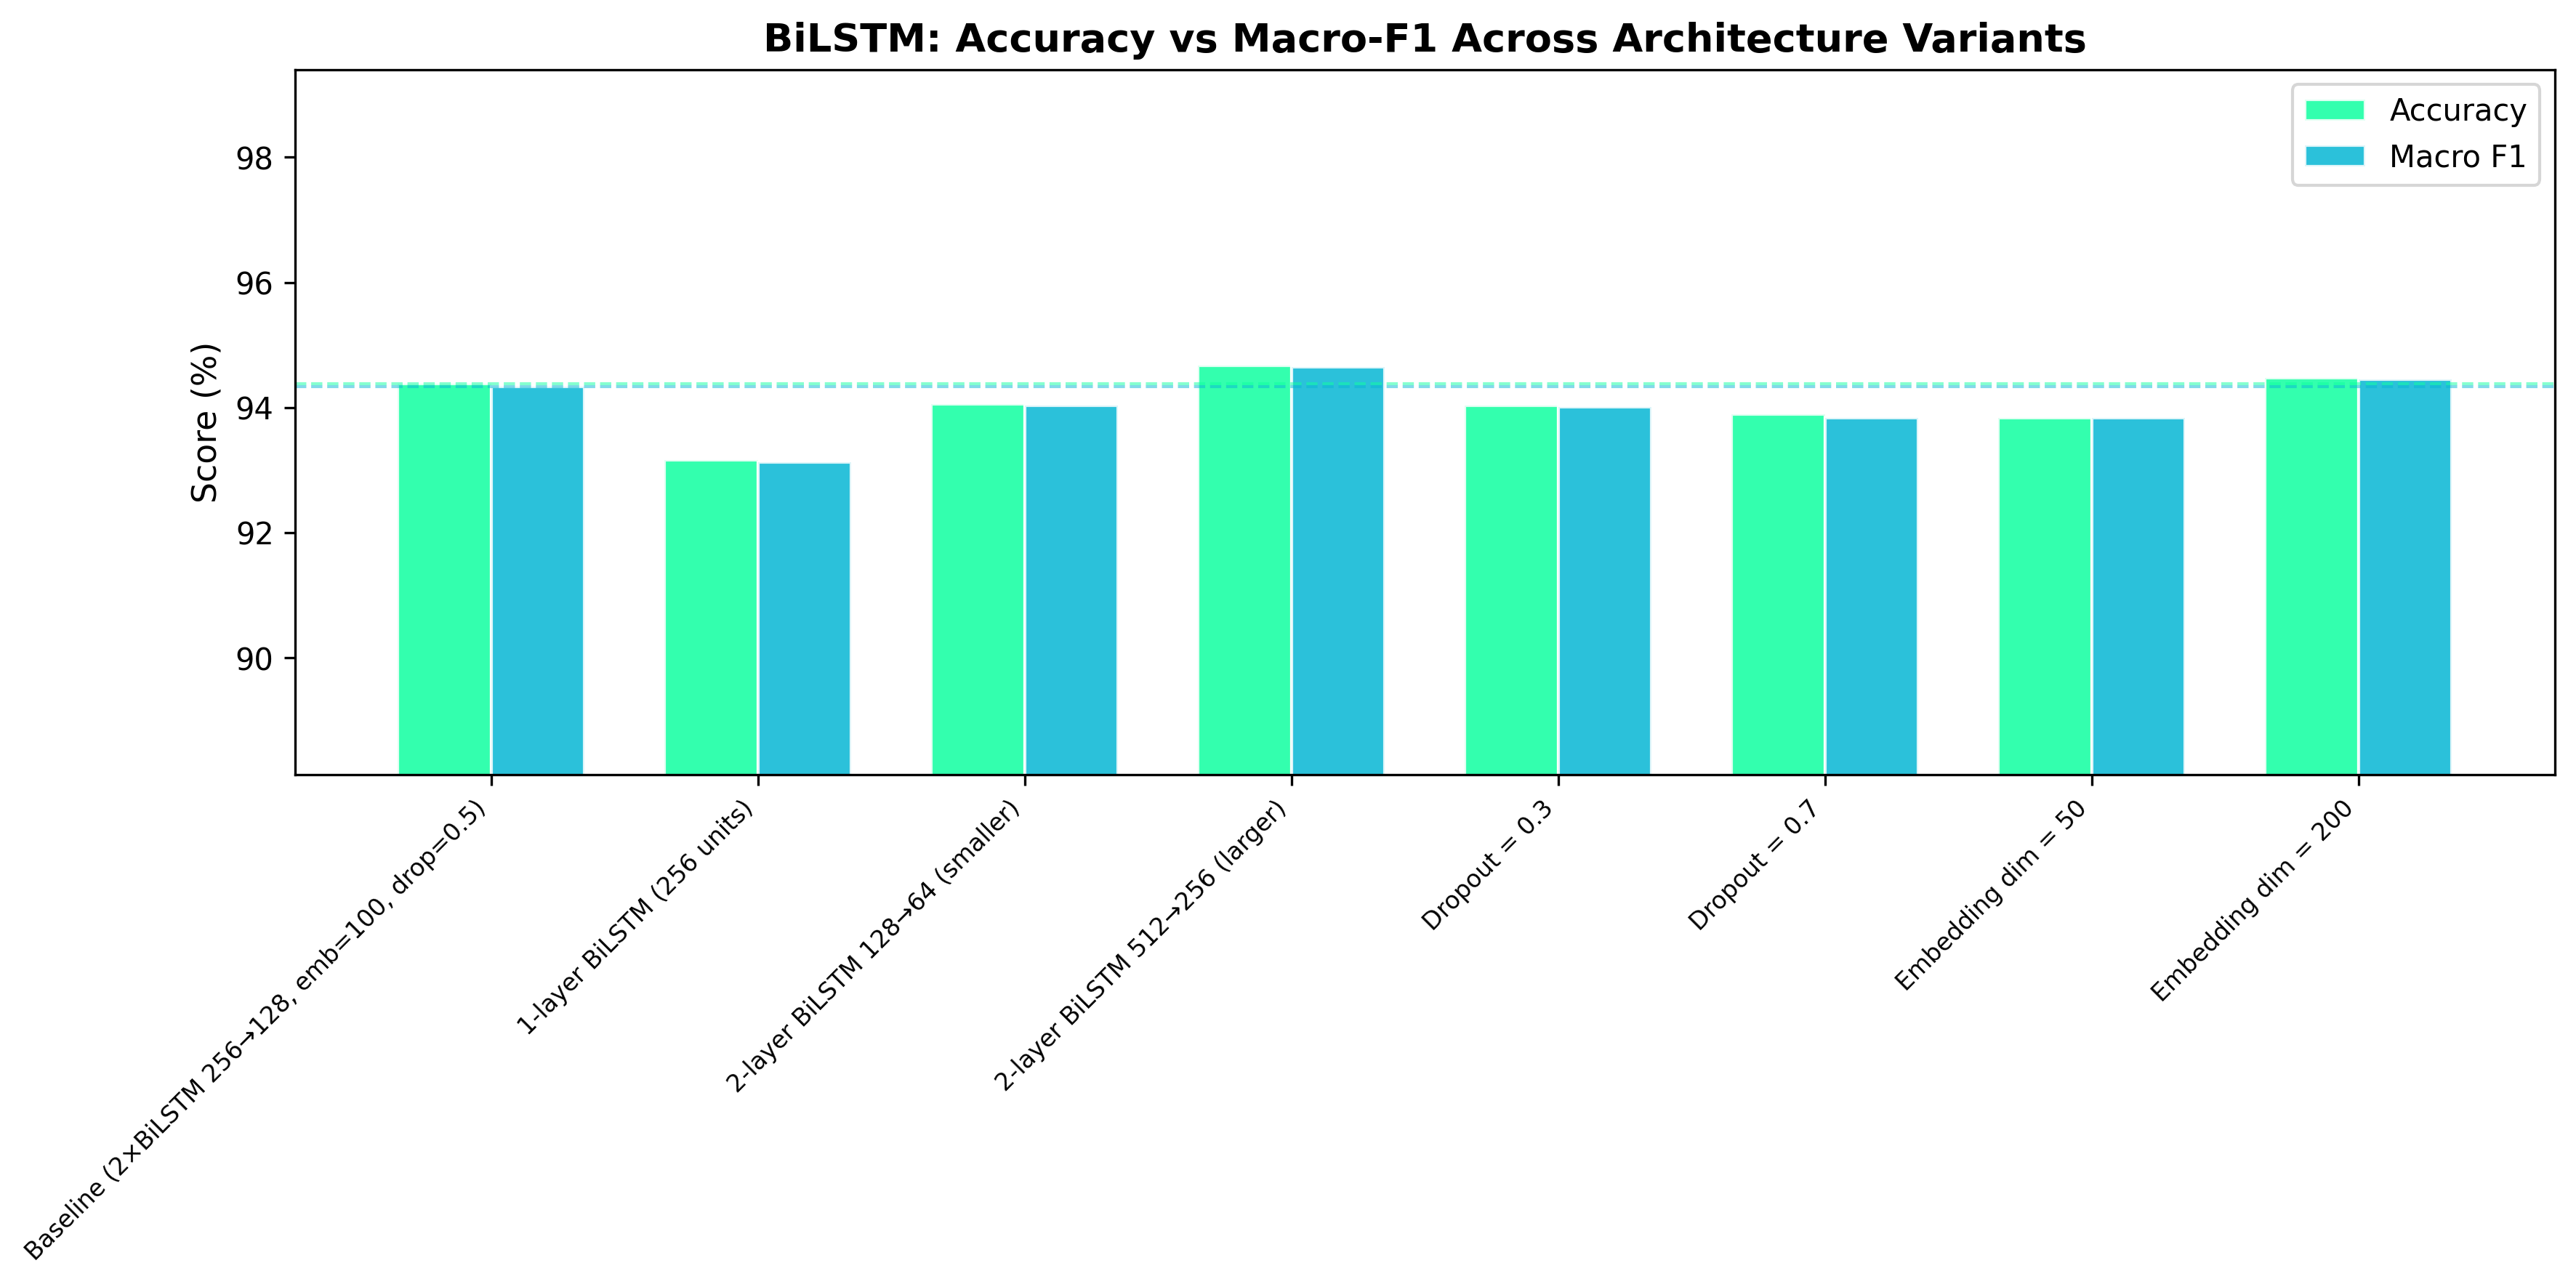
\includegraphics[width=0.85\linewidth]{figures/ablation_bilstm_f1.png}
\caption{BiLSTM ablation --- Accuracy and Macro-F1 across architecture variants. Reducing depth to a single layer causes the largest performance loss; the larger 512$\to$256 variant slightly exceeds the baseline.}
\label{fig:ablation_bilstm_f1}
\end{figure}
